\section{Evaluation}
Our evaluation has two goals. 1) We want to demonstrate that the code produced by \tool without additional optimization does not have any inexplicable performance differences than a state-of-the-art compiler like Clang. 2) We explore how \tool's internal representation can support a mix of affine and SSA-based transformation in the same compilation flow, and evaluate the potential benefits compared to existing source and compiler-based polyhedral tools.

%Our goal is twofold: First, we want to demonstrate that the code generated by \tool is on-par with the code generated by a state-of-the-art compiler like Clang (Section~\ref{sub:frontend}). Second, we wish to demonstrate the feasibility of utilizing existing polyhedral flows, especially research compilers, to process MLIR (Section~\ref{sub:polymer}).
%We are \emph{not} interested in using MLIR to produce better-optimized code than polyhedral flows.

\subsection{Experimental Setup}

We ran our experiments on an AWS \icode{c5.metal} instance with hyper-threading and Turbo Boost disabled. %(Table~\ref{table:arch}).
The system is Ubuntu 20.04 running on a dual-socket Intel Xeon Platinum 8275CL CPU at 3.0~GHz with 24 cores each, with 0.75, 35, 35.75~MB L1, L2, L3 cache per socket, respectively, and 256~GB RAM.
We ran all 30 benchmarks from PolyBench~\cite{polybench}, using the ``EXTRALARGE'' dataset. Pluto is unable to extract \scop from the \icode{adi} benchmark. We ran a total of 5 trials for each benchmark, taking the execution time reported by PolyBench; the median result is taken unless stated otherwise. Every measurement or result reported in the following sections refers to double-precision data. All experiments were run on cores 1-8, which ensured that all threads were on the same socket and did not potentially conflict with processes scheduled on core 0.

% \begin{table}
% \caption{Hardware setup.}
% \label{table:arch}
% \centering
% \resizebox{\columnwidth}{!}{%
% \begin{tabular}{lllll}
%     \toprule
%     \footnotesize{CPU} & 
%     \footnotesize{Clock rate} & 
%     \footnotesize{OS} & 
%     \footnotesize{RAM (GB)} & 
%     \footnotesize{L1/L2/L3 (MB)} \\ \midrule

%     \footnotesize{Intel Xeon Platinum 8275CL} & 
%     \footnotesize{3.0 GHz} & 
%     \footnotesize{Ubuntu 20.04} & 
%     \footnotesize{256} &
%     \footnotesize{1.5, 48, 71.5} \\ \bottomrule
% \end{tabular}
% }
% \end{table}

In all cases, we use two-stage compilation: (i) using \icode{clang} at \icode{-O3} excluding unrolling and vectorization; or \tool to emit LLVM IR from C; (ii) using \icode{clang} at \icode{-O3} to emit the final binary. As several optimizations are not idempotent, a second round of optimization can potentially significantly boost (and rarely, hinder) performance. This is why we chose to only perform vectorization and unrolling at the last optimization stage. Since \tool applies some optimizations at the MLIR level (e.g., mem2reg), we compare against the two-stage compilation pipeline as a more fair baseline (\textsc{Clang}). We also evaluate a single-stage compilation to assess the effect of the two-stage flow (\textsc{ClangSing}).

\subsection{Baseline Performance}
\label{sub:frontend}
\tool must generate code with runtime \emph{as close as possible} to that of existing compilation flows to establish a solid baseline. In other words, \tool should \emph{not introduce overhead nor speedup} unless explicitly instructed otherwise, to allow for measuring the effects of additional optimizations. We evaluate this by comparing the runtime of programs produced by \tool with those produced by Clang at the same commit (Apr 2021)\footnote{LLVM\,commit\,\icode{20d5c42e0ef5d252b434bcb610b04f1cb79fe771}}. Figure~\ref{fig:mlir_clang} summarizes the results with the following flows:
\begin{itemize}
  \item \textsc{Clang}: A compilation of the program using Clang, when running two stages of optimization;
  \item \textsc{ClangSing}: A compilation of the program using Clang, when running one stage of optimization;
  \item \textsc{MLIR-Clang}: A compilation flow using the \tool frontend and preprocessing optimizations within MLIR, but not running polyhedral scheduling nor postprocessing.
\end{itemize}

%To evaluate the similarity of \tool and Clang, we compute the percent difference of all benchmarks with a runtime greater than 0.05. The mean absolute-value percent difference is only 1.25\%, indicating that \tool indeed closely matches the performance of Clang.

%\begin{table}
{
%\caption{Geometric mean and standard deviation execution time of programs produced by \tool and Clang on Polybench EXTRALARGE double-precision single-thread. The rightmost column shows percent difference between Clang and \tool runtimes, with EXCL showing where a benchmark ran in below 0.05s.}
\caption{GeoMean and StdDev of program runtime with \tool and Clang on Polybench}
\label{table::clang_and_our_tool}

\centering
\footnotesize
\begin{tabular}{p{1.1cm}rp{0.01cm}rrp{0.01cm}rr}
    \toprule
    Benchmark     & Clang &$\pm$&$\sigma$   & \tool &$\pm$&$\sigma$ & \%-diff  \\ \midrule\rowcolor{aluminium1}
2mm&	63.191&$\pm$&	0.139&	62.117&$\pm$&	0.169 & 1.73\%\\
3mm&	106.955&$\pm$&	0.261&	104.705&$\pm$&	0.087& 2.15\%\\\rowcolor{aluminium1}
adi&	111.024&$\pm$&	0.215&	121.765&$\pm$&	0.203& -8.82\%\\
atax&	0.007&$\pm$&	<0.001&	0.007&$\pm$&	<0.001& EXCL\\\rowcolor{aluminium1}
bicg&	0.012&$\pm$&	<0.001&	0.006&$\pm$&	<0.001& EXCL\\
cholesky&	15.591&$\pm$&	0.017&	15.578&$\pm$&	0.007& 0.09\%\\\rowcolor{aluminium1}
correlation&	95.262&$\pm$&	0.020&	94.764&$\pm$&	0.065& 0.52\%\\
covariance&	95.283&$\pm$&	0.016&	94.769&$\pm$&	0.068& 0.54\%\\\rowcolor{aluminium1}
deriche&	1.686&$\pm$&	0.003&	1.669&$\pm$&	0.001& 1.03\%\\
doitgen&	5.123&$\pm$&	0.012&	4.920&$\pm$&	0.005& 4.12\%\\\rowcolor{aluminium1}
durbin&	0.017&$\pm$&	0.005&	0.015&$\pm$&	<0.001& EXCL\\
fdtd-2d&	25.803&$\pm$&	0.039&	25.879&$\pm$&	0.060& -0.30\%\\\rowcolor{aluminium1}
floyd-w.&	146.009&$\pm$&	0.061&	146.015&$\pm$&	0.052& 0.00\%\\
gemm&	8.467&$\pm$&	0.013&	8.626&$\pm$&	0.011& -1.83\%\\\rowcolor{aluminium1}
gemver&	0.160&$\pm$&	<0.001&	0.158&$\pm$&	<0.001& 1.27\%\\
gesummv&	0.024&$\pm$&	<0.001&	0.014&$\pm$&	<0.001& EXCL\\\rowcolor{aluminium1}
gramsch. &	152.444&$\pm$&	0.086&	152.254&$\pm$&	0.067& -0.12\%\\
heat-3d&	33.022&$\pm$&	0.127&	32.964&$\pm$&	0.028& 0.17\%\\\rowcolor{aluminium1}
jacobi-1d&	0.005&$\pm$&	0.002&	0.006&$\pm$&	0.002& EXCL\\
jacobi-2d&	24.149&$\pm$&	0.050&	24.952&$\pm$&	0.019& -3.22\%\\\rowcolor{aluminium1}
lu&	101.382&$\pm$&	0.386&	101.495&$\pm$&	0.388& -0.11\%\\
ludcmp&	99.538&$\pm$&	0.546&	99.155&$\pm$&	0.671& 0.39\%\\\rowcolor{aluminium1}
mvt&	0.146&$\pm$&	<0.001&	0.144&$\pm$&	<0.001& 1.27\%\\
nussinov&	133.654&$\pm$&	0.288&	133.811&$\pm$&	0.094& -0.12\%\\\rowcolor{aluminium1}
seidel-2d&	202.318&$\pm$&	0.015&	202.289&$\pm$&	0.001& 0.01\%\\
symm&	55.253&$\pm$&	0.071&	54.214&$\pm$&	0.030& 1.92\%\\\rowcolor{aluminium1}
syr2k&	70.523&$\pm$&	0.200&	70.359&$\pm$&	0.053& 0.23\%\\
syrk&	25.982&$\pm$&	0.265&	25.993&$\pm$&	0.177& -0.04\%\\\rowcolor{aluminium1}
trisolv&	0.012&$\pm$&	<0.001&	0.012&$\pm$&	<0.001& EXCL\\
trmm&	47.946&$\pm$&	0.211&	47.941&$\pm$&	0.369& 0.01\%\\ \bottomrule
\end{tabular}
}
\end{table}
%\begin{table}
{
%\caption{Geometric mean and standard deviation execution time of programs produced by \tool and Pluto on Polybench EXTRALARGE double-precision single-thread. The rightmost column shows the percent difference between \tool and Pluto runtimes with same exclusion rule as Table~\ref{table::clang_and_our_tool}. Pluto cannot compile the \icode{adi} benchmark.}
\caption{GeoMean and StdDev of program runtime with \tool and Pluto on Polybench.}
\label{table::polymer}

\footnotesize
\centering
\begin{tabular}{p{1.1cm}rp{0.01cm}rrp{0.01cm}rr}
    \toprule
Benchmark   & Pluto &$\pm$&$\sigma$   & \tool &$\pm$&$\sigma$ & \%-diff  \\ \midrule\rowcolor{aluminium1}
2mm           & 4.471  & $\pm$ & 0.017 & 4.258  & $\pm$ & 0.018 & 4.765\% \\
3mm           & 8.757  & $\pm$ & 0.026 & 7.731  & $\pm$ & 0.003 & 11.724\% \\
\rowcolor{aluminium1}
adi           & \multicolumn{7}{c}{Pluto fails to compile} \\
atax          & 0.011  & $\pm$ & 0.002 & 0.011  & $\pm$ & 0.001 & EXCL      \\
\rowcolor{aluminium1}
bicg          & 0.010  & $\pm$ & 0.001 & 0.006  & $\pm$ &<0.001 & EXCL      \\
cholesky      & 10.775 & $\pm$ & 0.056 & 11.285 & $\pm$ & 0.097 & -4.731\%  \\
\rowcolor{aluminium1}
correlation   & 4.153  & $\pm$ & 0.019 & 4.228  & $\pm$ & 0.003 & -1.822\%  \\
covariance    & 4.111  & $\pm$ & 0.018 & 4.253  & $\pm$ & 0.004 & -3.452\%  \\
\rowcolor{aluminium1}
deriche       & 1.771  & $\pm$ & 0.001 & 1.762  & $\pm$ & 0.001 & 0.571\%   \\
doitgen       & 1.869  & $\pm$ & 0.021 & 1.417  & $\pm$ & 0.010 & 24.192\%  \\
\rowcolor{aluminium1}
durbin        & 0.017  & $\pm$ & 0.005 & 0.015  & $\pm$ &<0.001 & EXCL      \\
fdtd-2d       & 21.717 & $\pm$ & 0.205 & 15.930 & $\pm$ & 0.073 & 26.627\%  \\
\rowcolor{aluminium1}
floyd-w.      & 380.402& $\pm$ & 0.694 & 345.460& $\pm$ & 0.569 & 9.186\%   \\
gemm          & 4.591  & $\pm$ & 0.036 & 5.110  & $\pm$ & 0.006 & -11.306\% \\
\rowcolor{aluminium1}
gemver        & 0.099  & $\pm$ & 0.001 & 0.097  & $\pm$ &<0.001 & 2.356\%   \\
gesummv       & 0.035  & $\pm$ & 0.001 & 0.014  & $\pm$ &<0.001 & EXCL      \\
\rowcolor{aluminium1}
gramschm.     & 14.647 & $\pm$ & 0.172 & 14.730 & $\pm$ & 0.171 & -0.569\%  \\
heat-3d       & 28.723 & $\pm$ & 0.037 & 29.752 & $\pm$ & 0.033 & -3.581\%  \\
\rowcolor{aluminium1}
jacobi-1d     & 0.008  & $\pm$ & 0.003 & 0.010  & $\pm$ & 0.002 & EXCL      \\
jacobi-2d     & 17.322 & $\pm$ & 0.077 & 22.616 & $\pm$ & 0.217 & -30.561\% \\
\rowcolor{aluminium1}
lu            & 10.667 & $\pm$ & 0.034 & 10.274 & $\pm$ & 0.049 & 3.689\%   \\
ludcmp        & 98.916 & $\pm$ & 0.249 & 98.803 & $\pm$ & 0.716 & 0.114\%   \\
\rowcolor{aluminium1}
mvt           & 0.084  & $\pm$ & 0.001 & 0.083  & $\pm$ &<0.001 & 0.196\%   \\
nussinov      & 124.424& $\pm$ & 0.122 & 124.062& $\pm$ & 0.147 & 0.291\%   \\
\rowcolor{aluminium1}
seidel-2d     & 237.186& $\pm$ & 0.028 & 164.344& $\pm$ & 0.003 & 30.711\%  \\
symm          & 53.952 & $\pm$ & 0.037 & 53.921 & $\pm$ & 0.086 & 0.058\%   \\
\rowcolor{aluminium1}
syr2k         & 9.946  & $\pm$ & 0.008 & 10.006 & $\pm$ & 0.008 & -0.605\%  \\
syrk          & 5.374  & $\pm$ & 0.005 & 5.328  & $\pm$ & 0.003 & 0.855\%   \\
\rowcolor{aluminium1}
trisolv       & 0.024  & $\pm$ &<0.001 & 0.024  & $\pm$ &<0.001 & EXCL      \\
trmm          & 2.079  & $\pm$ & 0.025 & 2.215  & $\pm$ & 0.001 & -6.550\%  \\
\bottomrule
\end{tabular}
}
\end{table}
\begin{figure*}
\centering
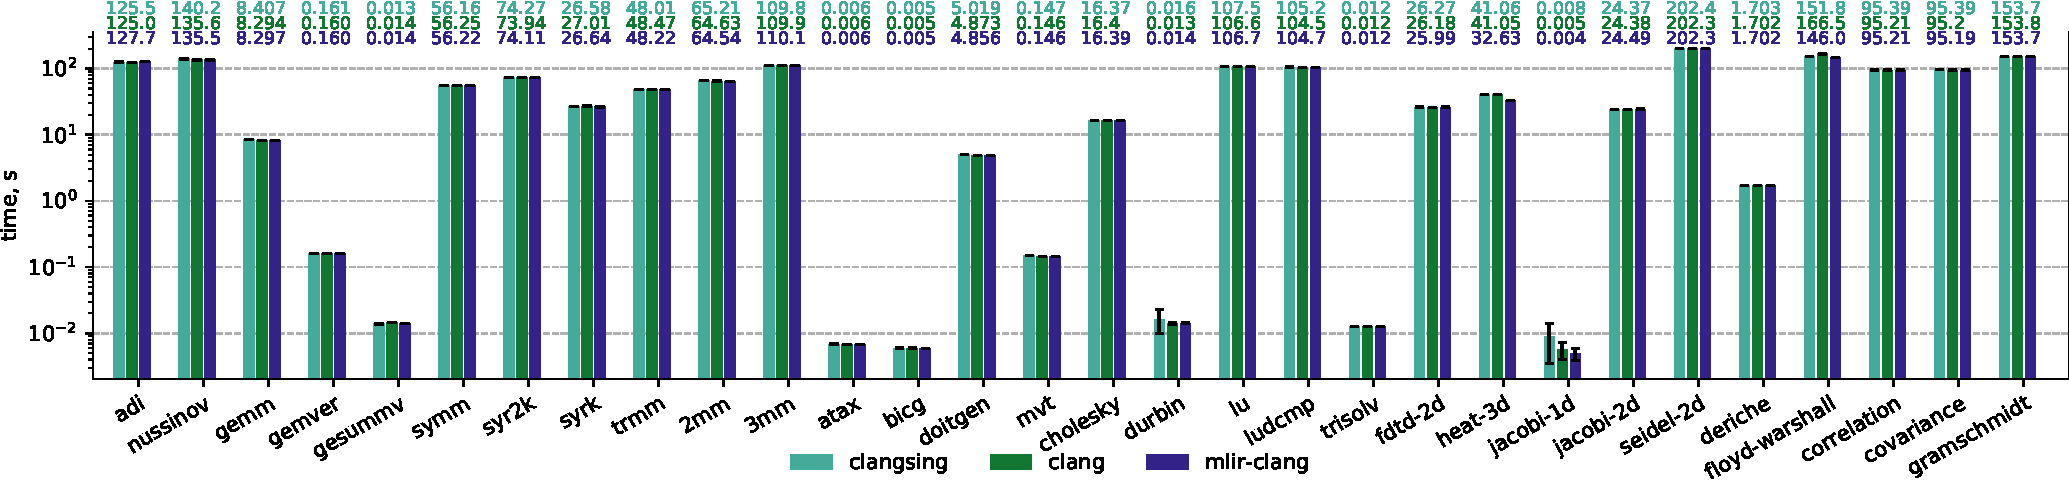
\includegraphics[width=\textwidth]{images/times.pdf}
\caption{Mean and 95\% confidence intervals (log scale) of program run time across 5 runs of Polybench in \textsc{Clang}, \textsc{ClangSing} and \textsc{MLIR-Clang} configurations, lower is better. The run times of code produced by \tool without optimization is comparable to that of Clang. No significant variation is observed between single and double optimization. Short-running \icode{jacobi-1d} shows high intra-group variation.}
\label{fig:mlir_clang}
\end{figure*}

\subsection{Compilation Flows}
\label{sub:polymer}

We compare \tool with a source-level and an IR-level optimizer (Pluto and Polly) in the following configurations:
\begin{itemize}
  \item \textsc{Pluto}: Pluto compiler auto-transformation~\cite{Bondhugula2008Pluto} using \polycc\footnote{Pluto commit \icode{dae26e77b94b2624a540c08ec7128f20cd7b7985}} with \icode{--noparallel} and \icode{--tile} flags;
  \item \textsc{PlutoPar}: Same as above but with \icode{--parallel} flag;
  \item \textsc{Polly}: Polly~\cite{grosser.ppl.2012} LLVM passes with affine scheduling and tiling, and no pattern-based optimizations~\cite{gareev_polly};
  \item \textsc{PollyPar}: Same as above with auto-parallelization;
  \item \textsc{Polygeist}: Our flow with Pluto and extra transforms;
  \item \textsc{Polygeistpar}: Same as above but with \icode{--parallel} Pluto schedule, \tool parallelization and reductions.
\end{itemize}

Running between source and LLVM IR levels, we expect \tool to benefit from both worlds, thus getting code that is on par or better than competitors.\wmnote{a bit concerned re, see email.} When using Pluto, both standalone and within \tool, we disable the emission of vectorization hints and loop unrolling to make sure both transformations are fully controlled by the LLVM optimizer, which also runs in Polly flows. We run Polly in the latest stage of Clang compilation, using \icode{--mllvm -polly} and additional flags to enable affine scheduling, tiling and parallelization as required. Polly is taken at the same LLVM commit as Clang. We disable pattern-based optimizations~\cite{gareev_polly} that are not available elsewhere.
Figures~\ref{fig:seq_speedups} and~\ref{fig:par_speedups} summarize the results for sequential and parallel flows, respectively.
%and require Polly to ignore its profitability heuristic as Pluto does not have an equivalent.  %Figures~\ref{fig:seq_speedups} and~\ref{fig:par_speedups} summarize the results for sequential and parallel flows, %respectively.
%By taking the mean absolute-value of the performance differences of all the benchmarks that have greater than 0.05 sec runtime, we find \tool has 7.76\% percentage different in runtime compared with Pluto. We will discuss the performance difference in Section~\ref{sec:perf_analysis}
%We do not compare \tool with Polly for now since Polly uses a modified version of the Pluto algorithm, making it difficult for an apple-to-apple comparison between them.

\begin{figure*}
  \centering
  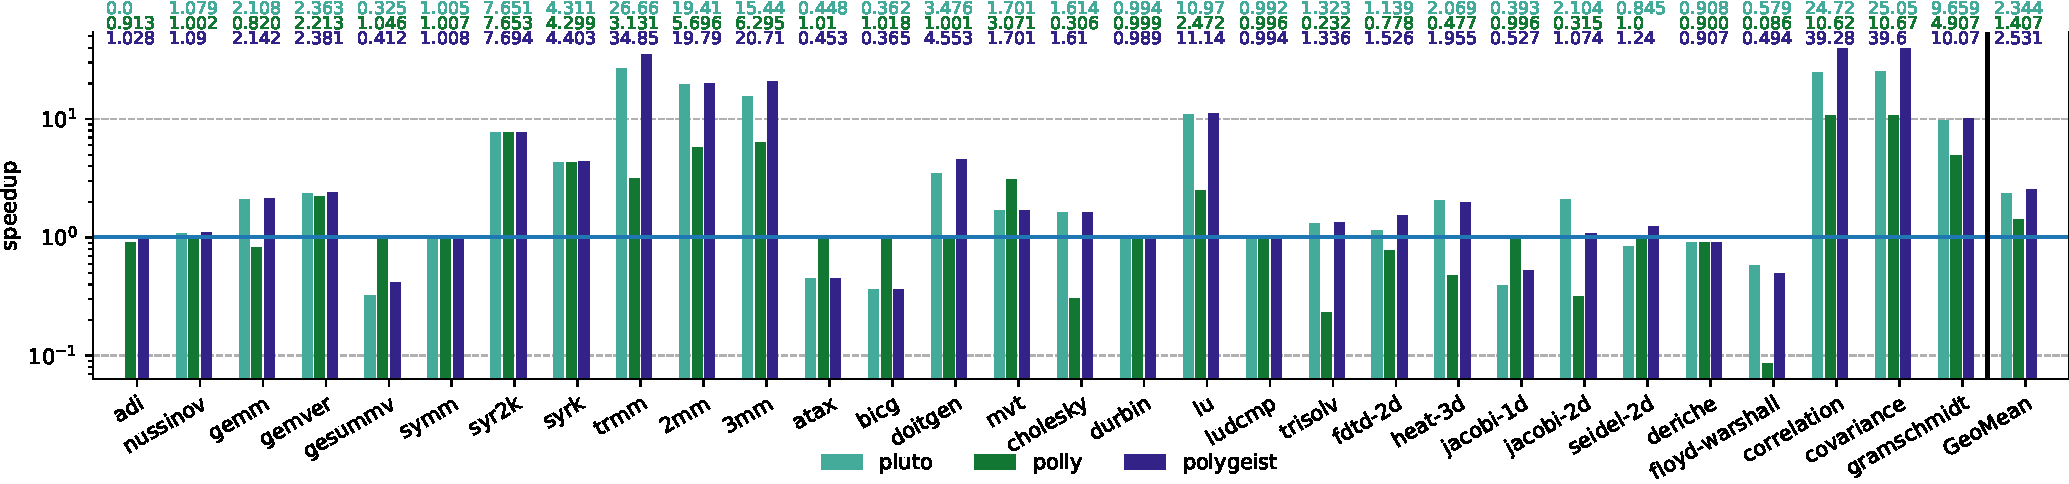
\includegraphics[width=\textwidth]{images/seq_speedups.pdf}
  \caption{Median speedup over \textsc{Clang} for sequential configurations (log scale), higher is better. \tool outperforms  (\toolseqspeedup geomean speedup) both Pluto (\plutoseqspeedup) and Polly (\pollyseqspeedup) on average. Pluto can't process \icode{adi}, which is therefore excluded from summary statistics.}
  \label{fig:seq_speedups}
\end{figure*}

\begin{figure*}
  \centering
  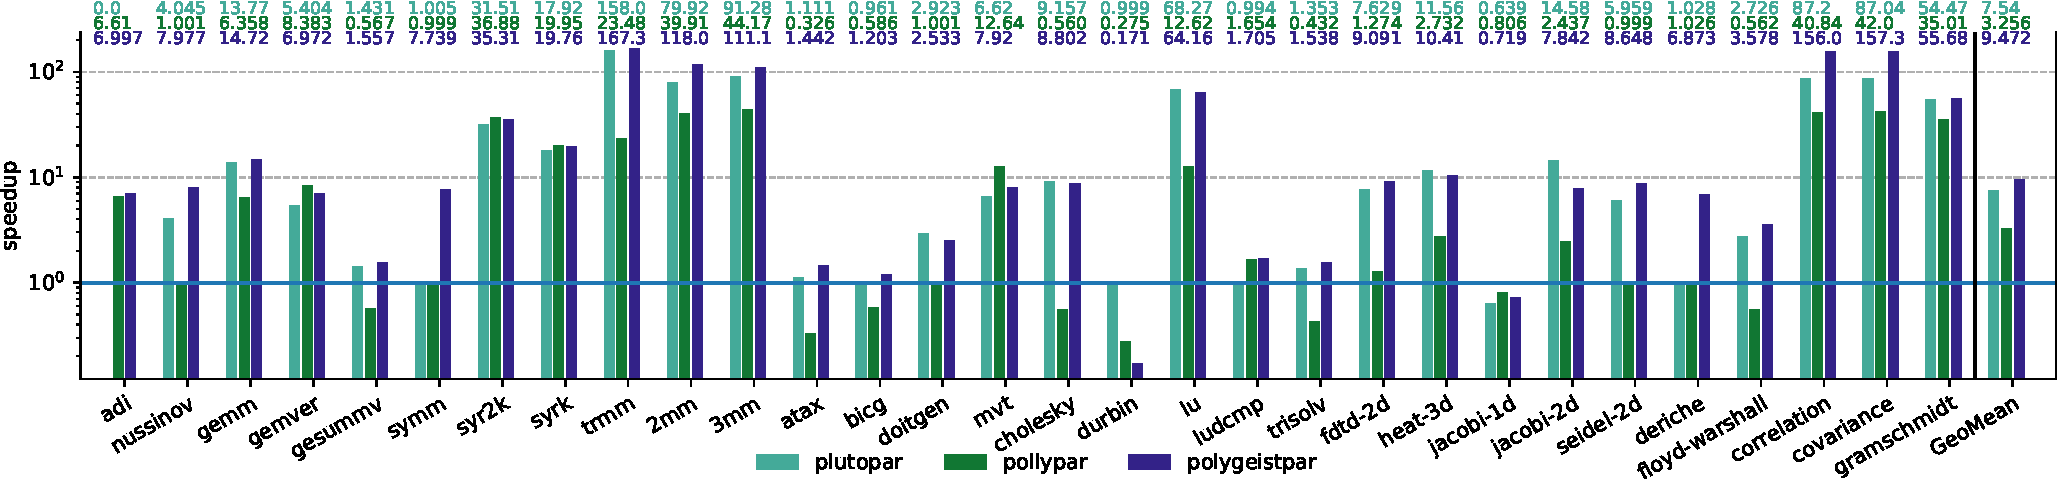
\includegraphics[width=\textwidth]{images/par_speedups.pdf}
  \caption{Median speedup over \textsc{Clang} for parallel configurations (log scale), higher is better. \tool outperforms  (\toolparspeedup geomean speedup) both Pluto (\plutoparspeedup) and Polly (\pollyparspeedup) on average. Pluto can't process \icode{adi}, which is therefore excluded from summary statistics.}
  \label{fig:par_speedups}
\end{figure*}

\section{Performance Analysis}
\subsection{Benchmarking}
The transformation of reduction loops, in particular parallelization, may result in a different order of partial result accumulation. This is not allowed under IEEE~754 semantics, but is supported by compilers with \icode{-ffast-math} option.
%, which we assume enabled.

%\az{List the benchmarks where it mattered and explain what we do to fix that.}

We found that Polybench allocation function hinders Clang/LLVM alias analysis, negatively affecting performance in, e.g., \icode{adi}. Therefore, we modified all benchmarks to use \icode{malloc} that is known to produce non-aliasing pointers.

%Finally, we found that the custom allocator used by Polybench had a nontrivial impact on the runtime of the kernel, particularly on the \icode{adi} test. This partially stems from the implementation of the allocation itself and LLVM's optimization pipeline assuming that calls to \icode{malloc} do not alias with existing allocations. To maximize the fairness of the evaluation, all flows were modified to use a standard \icode{malloc} as its memory allocation function.

\subsection{Baseline Comparison}
We did not observe a significant difference between the runtimes of \textsc{Clang} and \textsc{ClangSing} configurations, with a geometric mean of $0.43\%$ symmetric difference\footnote{Symmetric difference is computed as $2 \cdot |a - b| / (a + b)$.} across benchmarks.\wmnote{would consider removing explanation here, see email.} Therefore, we only consider \textsc{Clang} as baseline throughout the remainder of this paper. We did not observe a significant difference between the runtimes of \textsc{Clang} and \textsc{MLIR-Clang} configurations either, with a geometric mean of $0.24\%$ symmetric difference.

We found a variation in runtimes of short-running benchmarks, in particular \icode{jacobi-1d}. This can be attributed to the interaction with the data initialization and benchmarking code, and with other OS processes. Excluding the benchmarks running in under $0.05$s (\icode{jacobi-1d}, \icode{gesummv}, \icode{atax}, \icode{bicg}) from the analysis, we obtain $0.32\%$ and $0.17\%$ geomean symmetric differences respectively for the two comparisons above. These results suggest that our flow has no unexplained (dis)advantages over the baseline.

%The only benchmark with a nontrivial performance difference between \tool and Clang is the \icode{adi} test. This gap exists for two reasons: differences in allocation, and loop reversal. Specifically, compiling Polybench with Clang results in the use of a custom allocator, whereas using \tool, this results in a \memref allocation which is lowered to a \icode{malloc}. This difference in allocation function accounts for 48\% of the gap. The remaining gap exists because LLVM can strength reduce a specific load for the IR generated by Clang but not MLIR. LLVM cannot recognize this property in a reversed loop and consequently cannot perform the optimization. A future version of LLVM should permit this optimization. 

%Throughout benchmarking, we also found various behaviors of note. \tool supports the ability to compile two source files directly by producing a single MLIR module with all of the necessary functions. This is distinct from Clang, which will produce two LLVM modules that are eventually linked together. For our current benchmarks we strive to emulate the behavior of Clang by compiling the test file with \tool (e.g., nussinov.c) and linking it with timing utility code (polybench.c) using Clang. An earlier version of our pipeline, however, compiled both the timing utility code and benchmark together with \tool directly. For almost all benchmarks, this did not make a difference. But for the floyd-warshall test, we saw an 8\% reduction in performance by using a single module. An investigation into this found that interprocedural constant propagation between the utility and benchmark code allowed for significant optimization of floyd-warshall.

%Another crucial component of generating accurate code was ensuring that the code emitted by \tool had the same LLVM DataLayout and Target as that emitted by Clang natively. \tool directly parses these and marks the MLIR appropriately when it lowers Clang AST. This is not sufficient, however, as MLIR currently will not propagate the DataLayout to the eventual LLVM. This is problematic as it will result in LLVM not performing vectorization in the same way. We modified MLIR to ensure this information is propagated successfully throughout all stages of the pipeline.

\subsection{Performance Differences in Sequential Code}\label{sec:perf_analysis}
Overall, \tool leads to larger speedups, with \toolseqspeedup geometric mean, than both Pluto (\plutoseqspeedup) and Polly (\pollyseqspeedup), although improvements are not systematic. Some difference between \tool and Polly is due to the employed polyhedral schedulers, e.g., in \icode{lu} and \icode{mvt}. \tool produces code faster tha both Pluto and Polly in \icode{2mm}, \icode{3mm} and others thanks to statement splitting, see Section~\ref{sec:splitcase}.

Given identical statements and schedules, codegen-level optimization accounts for other performance difference. \icode{seidel-2d} is the clearest example: Pluto executes $2.7\!\cdot\!10^{11}$ more integer instructions than \tool. Assuming these to be index/address computations, a mix of \icode{add} (throughput $1/2$ or $1/4$) and \icode{imul/shl} (thoughput $1$), we can expect a $\approx 59$s difference at 3GHz, consistent with experimental observations. \tool optimizes away a part of those in its post-optimization phase and emits homogeneous address computation from \memref with proper machine size type, enabling more aggressive bound analysis and simplification in the downstream compiler. Conversely, \icode{jacobi-2d} has poorer performance because \tool gives up on simplifying CLooG code, with up to 75 statement copies in 40 branches, for compiler performance reasons, as opposed to Clang that takes up to 5s to process it but results in better vectorization. Further work is necessary to address this issue by emitting vector instructions directly from \tool.

%Even with the same schedule, differences in code generation may lead to performance differences. More specifically, the exact shape of domain relations fed to CLooG (e.g., the inclusion of constraints on parameters into the \emph{domain}) significantly changes the final AST. This can be addressed through a finer-grain control over the AST generation process~\cite{grosser2015polyhedral}. Furthermore, MLIR's \icode{index} type converts to the proper machine index type, which, in conjunction with automatic simplification of affine forms in MLIR, enables a more aggressive bound analysis in the downstream compiler.

%\todo{there was a nice analysis for seidel-2d, but we need new numbers here!}
%Consider, for example, \icode{seidel-2d}. \tool produces $30\%$ faster code. Analyzing the execution with \icode{perf}, we observe that both Pluto and \tool issue $143 \cdot 10^9$ FP instructions, but Pluto issues $585 \cdot 10^9$ total instructions as opposed to $254 \cdot 10^9$ by \tool. These instructions are related to control flow and address computations. Assuming a mix of \icode{add} (throughput $1/3$) and \icode{imul} (throughput $2$), the extra $331 \cdot 10^9$ instructions can comfortably explain the performance difference of 73s when running at 3GHz ($219 \cdot 10^9$ extra cycles). This can be attributed to the \memref representation that emits homogeneous, LLVM-friendly address computations.

\subsection{Performance Differences In Parallel Code}\label{sec:parallel_perf_analysis}
Similarly to sequential code, some performance differences are due to different schedulers. For example, in \icode{cholesky} and \icode{lu}, both Pluto and \tool outperform Polly, and the remaining gap can be attributed to codegen-level differences. Conversely, in \icode{gemver} and \icode{mvt} Polly has a benefit over both Pluto and \tool. On \icode{ludcmp} and \icode{syr(2)k}, SSA-level optimizations let \tool produce code which is faster than Pluto and at least as fast as Polly. These results demonstrate that \tool indeed leverages the benefits of both the affine and SSA-based optimizations.

\tool is the only flow that obtains speedup on \icode{deriche} ($6.9\times$) and \icode{symm} ($7.7\times$). Examining the output code, we observe that only \tool manages to parallelize these two benchmarks. Considering the input code in Figure~\ref{fig:deriche}, one can observe that the \icode{i} loop reuses the \icode{ym1} variable, which is interpreted as parallelism-preventing loop-carried dependency by polyhedral schedulers. \tool performs its own parallelism analysis after promoting \icode{ym1} to an SSA register (carried by the \icode{j} loop) whose use-def range does not prevent parallelization.

\begin{figure}
  \centering
  \begin{tabular}{p{0.44\linewidth}p{0.52\linewidth}}
  {\scriptsize
  \begin{lstlisting}[language=c]
for (i=0; i<_PB_W; i++){
  ym1 = SCALAR_VAL(0.0);
  // ...
  for (j=0; j<_PB_H; j++){
    ym1 = y1[i][j];
  /*...*/ }
}
  \end{lstlisting}
  }&
  {\scriptsize
  \begin{lstlisting}[language=llvm]
%z = constant 0.0 : f64
affine.parallel %i = ... {
  affine.for %j = ...
  iter_args(%ym1=%z)->f64 {
    %0=affine.load %y1[%i,%j]
    // ...
    affine.yield %0
}}
  \end{lstlisting}
  }
  \end{tabular}
  \vspace{-2em}
  \caption{Excerpt from the \icode{deriche} benchmark. The outer loop reuses \icode{ym1} which makes it appear non-parallel to affine schedulers (left). \tool detects parallelism thanks to its mem2reg optimization, reduction-like loop-carried \icode{\%ym1} value detection and late parallelization (right).}
  \label{fig:deriche}
\end{figure}

Similarly, the \tool parallelizer identifies two benchmarks with parallel reduction loops that are not contained in other parallel loops: \icode{gramschmidt} and \icode{durbin}. \icode{gramschmidt} benefits from a $56\times$ speedup with \tool, compared to $34\times$ with Polly and $54\times$ with Pluto. \icode{durbin} sees a $6\times$ slowdown since the new parallel loop has relatively few iterations and is nested inside a sequential loop, leading to synchronization costs that outweigh the parallelism benefit. Section~\ref{sec:durbin} explores the \icode{durbin} benchmark in more detail. Polybench is a collection of codes (mostly) known to be parallel and, as such, has little need for reduction parallelization on CPU where one degree of parallelism is sufficient. When targeting inherently target architectures as GPUs, however, exploiting reduction parallelism could be vital for achieving peak performance~\cite{larsen2017strategies,reduction_drawing}.

\subsection{Case Study: Statement Splitting}\label{sec:splitcase}
We identified 5 benchmarks where the statement splitting heuristic applied: \icode{2mm}, \icode{3mm}, \icode{correlation}, \icode{covariance} and \icode{trmm}. To assess the effect of the transformation, we executed these benchmarks with statement splitting disabled, suffixed with \icode{-nosplit} in Figure~\ref{fig:split_case}. In sequential versions, \icode{2mm} is $4.1\%$ slower (3.13s vs 3.26s), but the other benchmarks see speedups of $25\%$, $50\%$, $51\%$ and $27\%$, respectively. For parallel versions, the speedups are of $36\%$, $20\%$, $44\%$, $40\%$ and $-9\%$ respectively.

Examination of polyhedral scheduler outputs demonstrates that it indeed produced the desired schedules. For example, in the \texttt{correlation} benchmark which had the statement \icode{A[i][j] += B[k][i]*B[k][j]}
%original C statement
%, split into \icode{S[k] += B[k][i]*B[k][j]} and \icode{A[i][j] += S[k]},
\tool was able to find the $(k, i, j)$ loop order after splitting.
%exploiting temporal locality for \icode{B[k][i]} and spatial locality for \icode{B[k][j]}.
Using hardware performance counters on sequential code we confirm that the overall cache miss ratio has indeed decreased by $75\%, 50\%, 20\%, 27\%,$ and $-26\%$, respectively. However, the memory traffic estimated by the number of bus cycles has \emph{increased} by $9\%$ for \icode{2mm}, and decreased by $18\%, 32\%,$ $32\%$, and $21\%$ for the other benchmarks. This metric strongly correlates with the observed performance difference in the same run ($r\!\!=\!\!0.99,  p=3\!\cdot\!10^{-11}$). This behavior is likely due to the scheduler producing a different fusion structure, e.g., not fusing outermost loops in \icode{2mm}, which also affects locality. Similar results can be observed for parallel code.  Further research is necessary to exploit the statement splitting opportunities, created by \tool, and interplay with fusion.

\begin{figure}
  \centering
  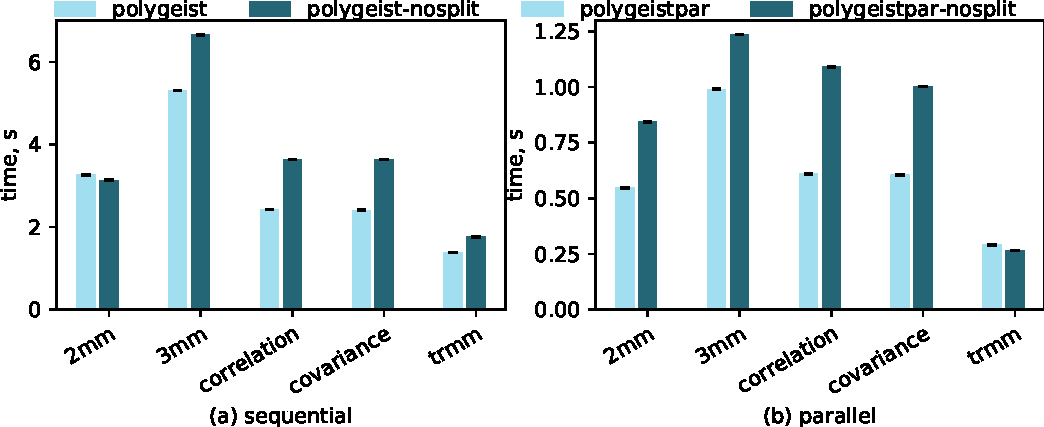
\includegraphics[width=\linewidth]{images/split.pdf}
  \caption{Mean and 95\% confidence intervals of run time across 5 runs of Polybench where statement splitting is applicable (Section~\ref{sec:stmt_splitting}), lower is better. It results in faster run time (geomean $1.28\times$ sequential, $1.39\times$ parallel speedup) except for sequential \icode{2mm} ($-4\%$) and parallel \icode{trmm} ($-9\%$).}
  \label{fig:split_case}
\end{figure}

\subsection{Case Study: Reduction Parallelization in {\tt durbin}}\label{sec:durbin}
In this benchmark, \tool uses its reduction optimization to create a parallel loop that other tools cannot. For the relatively small input run by default, $N=4000$ iterations inside another sequential loop with $N$ iterations, the overall performance decreases. We hypothesize that the cost of creating parallel threads and synchronizing them outweighs the benefit of the additional parallelism and test our hypothesis by increasing $N$. Considering the results in Figure~\ref{fig:durbin_case}, one observes that \tool starts yielding speedups ($>1$) for $N \geq 16000$ whereas Polly only does so at $N \geq 224000$, and to a much lesser extent: $6.62\times$ vs $1.01\times$. Without reduction parallelization, \tool follows the same trajectory as Polly. Pluto fails to parallelize any innermost loop and shows no speedup. This evidences in favor of our hypothesis and highlights the importance of being able to parallelize reductions.

\begin{figure}
  \centering
  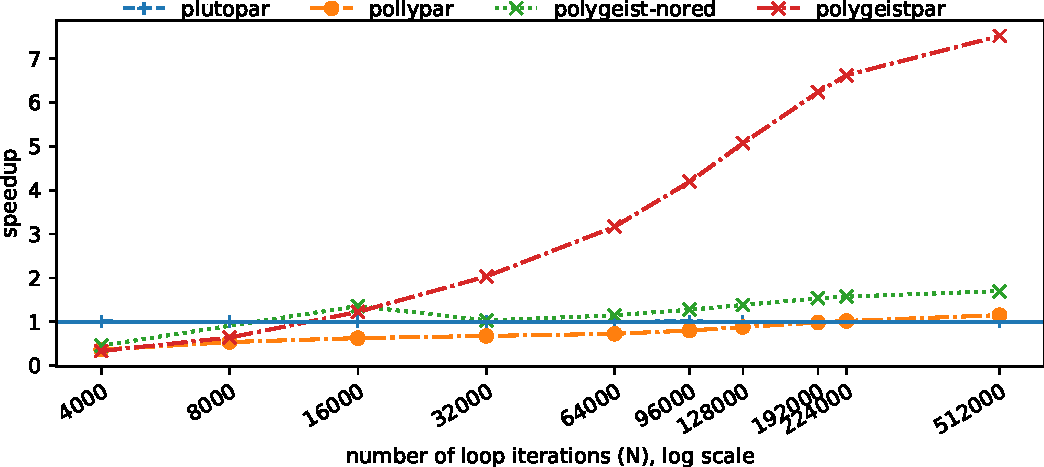
\includegraphics[width=\linewidth]{images/durbin.pdf}
  \caption{Reduction parallelization allows \textsc{{\tool}Par} to produce larger speedups in \texttt{durbin} and at smaller sizes than \textsc{PollyPar}, \textsc{{\tool}Par} without reduction support. \textsc{PlutoPar} fails to parallelize, hence no speedup.}
  \label{fig:durbin_case}
\end{figure}


